Le recours à l'hydrogène bas-carbone peut permettre de réduire le besoin en métal ou d'achever un bouclage énergétique. L'hydrogène bas-carbone est aujourd'hui très marginal dans le système énergétique mondial et l'évolution de sa part dans le système est très incertaine. Par conséquent, l'évolution du risque géopolitique autour de l'hydrogène est très incertaine.\\
\\
Cependant, il est possible que l'Europe devienne dans le besoin d'importer de l'hydrogène bas-carbone pour achever sa décarbonation. L'Allemagne envisage des parts significatives d'approvisionnement en hydrogène - de l'ordre de 10\% du mix de production - (\cite{rte_futurs_2022},\cite{world_energy_council_importations_2021}).\\
\\
D'autre part, plusieurs pays se positionnent pour devenir exportateur d'hydrogène comme le Maroc (\cite{bloomberg_morocco_2022}), les Emirats Arabes Unis (\cite{bloomberg_masdar_2023}), le Chili (\cite{us_government_chile_2021}), l'Australie (\cite{australian_government_growing_2022}).\\
Les enjeux géopolitiques dépendront de la diversité d'acteurs qui émergeront, des contrats qui lieront producteurs et acheteurs et la proportion des échanges d'hydrogène.
\begin{figure}[!b]
    \centering
    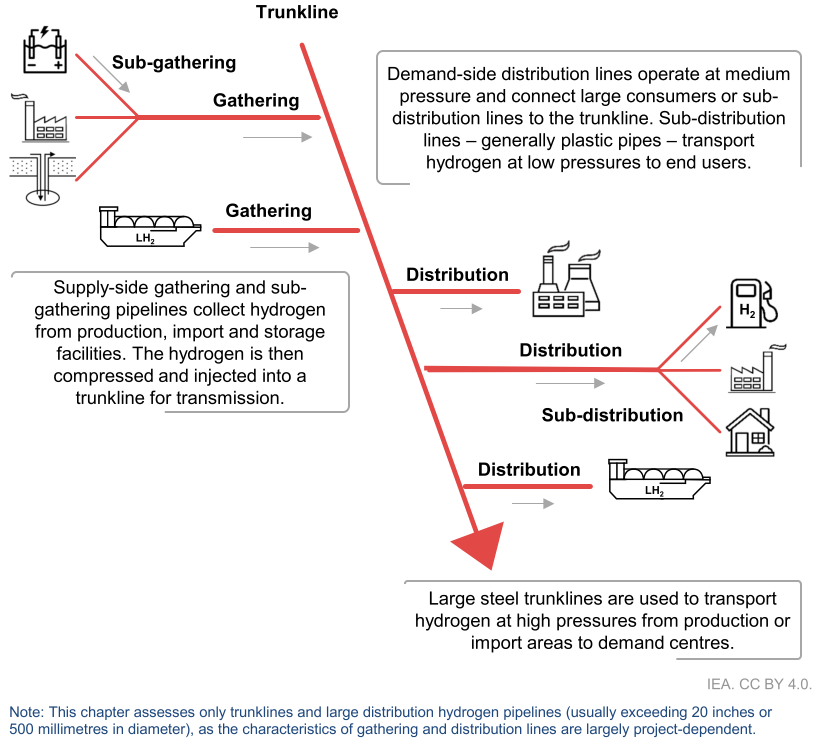
\includegraphics[width=0.9\textwidth]{Images/hydrogene/hydrogen_supply.png}
    \caption{Configuration du réseau d'approvisionnement en hydrogène (\cite{iea_energy_2023}}
    \label{fig:hydrogen_supply}
\end{figure}